%
% Este archivo es parte de un documento sobre OpenERP/Odoo creado
% y distribuido bajo licencia GNU Free Documen License v1.3.
%
% Para obtener la fuente e información más detallada, visite
% https://github.com/Gabriel-fm/oerp-manual
%
% Copyright (c) 2014 - Gabriel Franco
%

\chapter{Módulo de ventas}


%\section{Conceptos generales}

\section{Ventas}

La sección de ventas dentro del módulo de mismo nombre, es la sección a través de la 
cual se hará el seguimiento y control de las ventas de productos. Esto incluye tanto
las ventas probables como las ventas reales.

La estructuración de los menus sirves para tener una visión escalonada del punto en el que
se encuentra una posible venta. Cuando aparece una posible venta, según su origen (se verá
después) aparecerá un nuevo elemento en \textbf{Iniciativas} o \textbf{Oportunidades}. En
este punto se trata de un contacto con un posible cliente con el cuál se le va a dar forma a
la venta. En este punto aún no hay nada acordado con el mismo y sólo indica la existencia
de esa probable venta.

Cuando se ha tratado lo suficiente con el cliente y se ha dado forma a una oferta en la que el
cliente está interesado, el elemento creado en el apartado anterior (\emph{Iniciativas} o
\emph{ventas}) se escalará y pasará a formar un \textbf{Presupuesto} que se enviará al cliente
para su aprobación. En este punto se habla de una venta probable a falta de la aprobación del
cliente.

Si el presupuesto es aprobado, este pasará (escalandose, igual que anteriormente) a convertirse
en un \textbf{Pedido de venta}, el cuál es un elemento que permitirá al comercial al cargo
\emph{confirmar la venta} de un presupuesto, \emph{generar una factura} como en el apartado
\ref{contabilidad:factura} (que deberá ser aprobada por alguien
encargado de facturación) y \emph{generar un pedido de envío} en almacén (que será aprobado y
 gestionado por el encargado de almacén) que se puede ver en el la sección \ref{almacen:envio}.


\subsection{Clientes}
\label{ven:clientes}
Esta sección es el punto principal de acceso a los datos sobre los clientes. Al hacer click
sobre el mismo aparecerá el listado de clientes en su vista Kanban. En esta vista de datos
se pueden ver de un vistazo el nombre, datos de la empresa, correos, etiquetas y 
enlaces a las posibles oportunidades y ventas de los clientes. La figura \ref{ven:clikanban}
muestra la visión kanban. En los recuadros azules se pueden observar las etiquetas
y en algunos de ellos, bajo el nombre y/o las etiquetas se aprecian los enlaces a 
las oportunidades y ventas.

\begin{figure}[H]
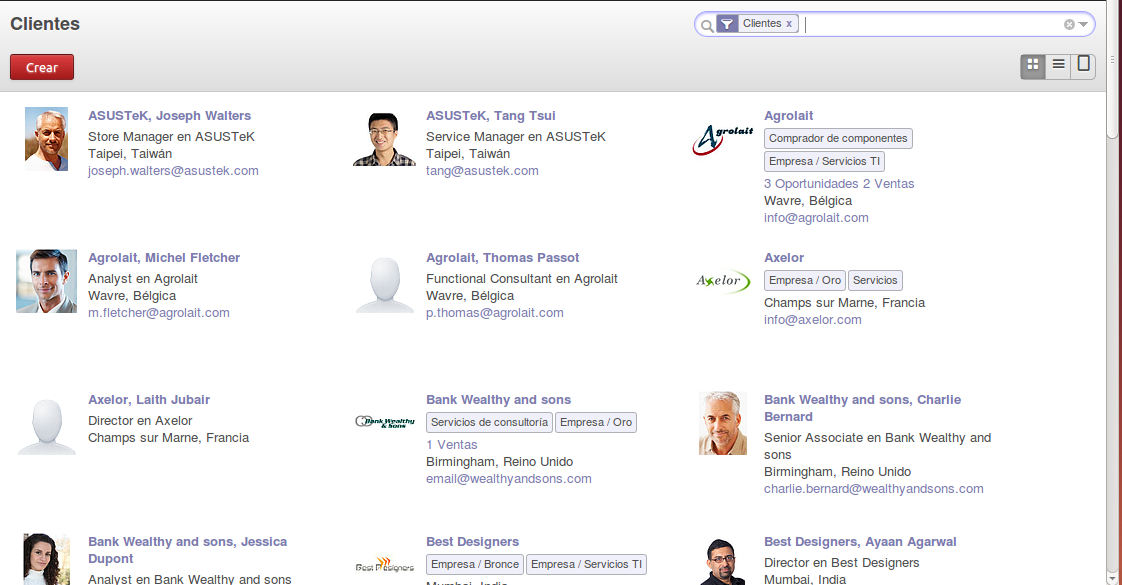
\includegraphics[width=\textwidth]{ventas/img/ven_clikanban.png}
\caption{Vista Kanban de clientes}
\label{ven:clikanban}
\end{figure}

Seleccionar uno de los clientes abrirá la ficha del mismo, pudiendo ver los datos del 
cliente que no estaban a la vista en la visión reducida. Esta ficha se compone de una
parte con los datos más "comunes" de los clientes y una serie de pestañas con información
adicional (contabilidad, ventas\ldots) sobre el mismo. La parte común se puede observar a
continuación en la figura \ref{ven:cliindividual}

\figura{ventas/img/ven_cliindividual.png}
{Información básica en la ficha de cliente}
{ven:cliindividual}


La mayoría de los campos son suficientemente autodescriptivos. Es necesario
mencionar otros no tan intuitivos. Por ejemplo, el cuadro de chequeo \textbf{¿Es una empresa?}
es utilizado para indicar si los datos que se están rellenado son de una empresa o 
de una persona en particular. Cuando este cuadro está marcado, se pueden crear nuevos
clientes y asociarlos a esta empresa. Para ello, los clientes que forman parte de esa
empresa, no tendrán marcado este cuadro de selección. Cuando este cuadro no se encuentra
seleccionado, aparece un nuevo campo que se denomina \emph{Compañia}, donde se indica
la compañia a la que pertenece el contacto.

Creando el contacto de la empresa y los contactos de personas relacionados con la misma
se consigue, por un lado, que la información de facturación y envío sea la de la empresa, 
evitando tener que rellenar varias veces la misma información en distintas fichas. Por otro
lado se organiza la información para que desde la ficha de la empresa se puedan observar también
los contactos que pertenecen a la misma, además de agilizar a la hora de realizar busquedas
el tener organizados los contactos con sus empresas.

En el área superior derecha se encuentran una serie de botones que permiten acceder a las reuniones, llamadas,
oportunidades y presupuestos y pedidos de compra de los clientes, presentando la lista de los elementos seleccionados
exclusivamente del cliente.

El área de \textbf{etiquetas} se utiliza para añadir identificadores a los clientes. Se utilizan
palabras cortas que identifiquen el área de trabajo de la empresa. Para clientes y empresas
que trabajen en joyería se debe añadir a los mismos la etiqueta \emph{joyería}, por ejemplo. La idea
es organizar todos los contactos con distintas etiquetas. Organizarlo de esta manera
optimiza los resultados a la hora de realizar busquedas.

En cuanto a las pestañas de la ficha de cliente se organizan en:

\subsubsection{Pestaña de Contactos}
En esta pestaña se pueden crear nuevos contactos que serán asociados directamente a la
empresa de la ficha. Si se crean nuevos contactos (en otro lugar, fuera de esta pestaña)
y se le asigna una compañia, esos contactos aparecerán aquí directamente.


\subsubsection{Pestaña de Notas Internas}
Permite almacenar información sobre el contacto, se guarda como texto en plano.


%\subsubsection{Pestaña de Información Mercantil}
\subsubsection{Pestaña de Ventas y Compras}
La información de esta pestaña es relativa a la información necesaria para realizar el contacto
con el cliente.

\begin{figure}[H]
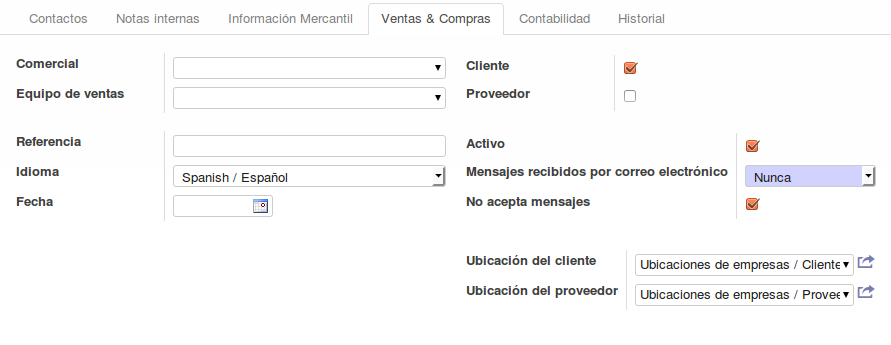
\includegraphics[width=\textwidth]{ventas/img/ven_cliventas.png}
\caption{Pestaña de Ventas y Compras en la ficha del cliente}
\label{ven:cliventas}
\end{figure}

\begin{itemize}
  \item \textbf{Comercial} -- Comercial al que se encuentra asignado este cliente
  \item \textbf{Equipo de ventas} -- Equipo de ventas en el que está asignado el cliente.
  \item \textbf{Referencia} -- Si se utiliza algún tipo de referencia a los clientes
        este campo es el lugar para ponerlo.
  \item \textbf{Idioma} -- Idioma del cliente. Según el idioma elegido, se enviarán los correos automáticos
        en el elegido.
  \item \textbf{Fecha} -- Permite almacenar una fecha. Según las necesidades del usuario.
  \item \textbf{Cliente/Proveedor} -- Según lo seleccionado en estos campos, se interpretará la información
        del contacto como un cliente o un proveedor. No es excluyente, es posible que los contactos sean
        proveedores y clientes al mismo tiempo.
  \item \textbf{Activo} -- Indica si el cliente/proveedor está activo. Si no seencuentra activo
        la información está almacenada, pero no se mostrará el cliente a menos que se busque de manera más
        específica.
  \item \textbf{No acepta mensajes} -- Indicador de si el cliente desea o no recibir correos.
  \item \textbf{Ubicaciones} -- Si se utilizan ubicaciones específicas en almacen para los datos de este cliente
        han de especificarse aquí.
\end{itemize}


\subsubsection{Pestaña de Contabilidad}
Los datos específicos sobre contabilidad del cliente se almacenan en esta pestaña.

Los distintos campos son autoexplicativos aunque cabe recalcar que la información del NIF debe introducirse
\textbf{en formato europeo}, es decir, con el prefijo de dos letras del país, la letra del NIF y el número. Para un NIF
español el formato sería con el prefijo ES de España, por ejemplo: ESA43683955 

Si al cobrar a un cliente se quiere almacenar la información de la transacción en un cuenta de contabilidad
43 específica, debe añadirse aquí (por ejemplo, para el primer cliente la cuenta sería 43000001)
De igual manera se trata la \emph{Cuenta a pagar}.

\begin{figure}[H]
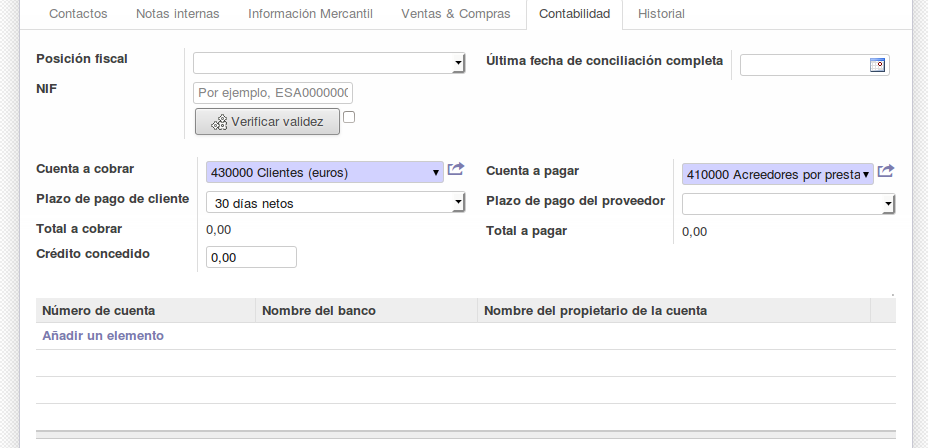
\includegraphics[width=\textwidth]{ventas/img/ven_clicontablidad.png}
\caption{Pestaña de Contabilidad en la ficha del cliente}
\label{ven:clicontabilidad}
\end{figure}



\subsubsection{Pestaña de Historial} 
La pestaña de historial almacena el listado de reclamaciones del cliente. Desde este
mismo punto se pueden añadir nuevas reclamaciones, pero es recomendable añadirlas desde su
sección.


\subsection{Iniciativas}
\label{iniciativas}
Las iniciativas representan clientes y ventas potenciales. Esto quiere decir que una iniciativa no crea una oportunidad de venta real
hasta que se califique si la iniciativa es interesante o no.

Se puede configurar OpenERP para que se creen iniciativas por cada correo recibido en alguna dirección de correo en concreto como info@suempresa.com.


\begin{figure}[H]
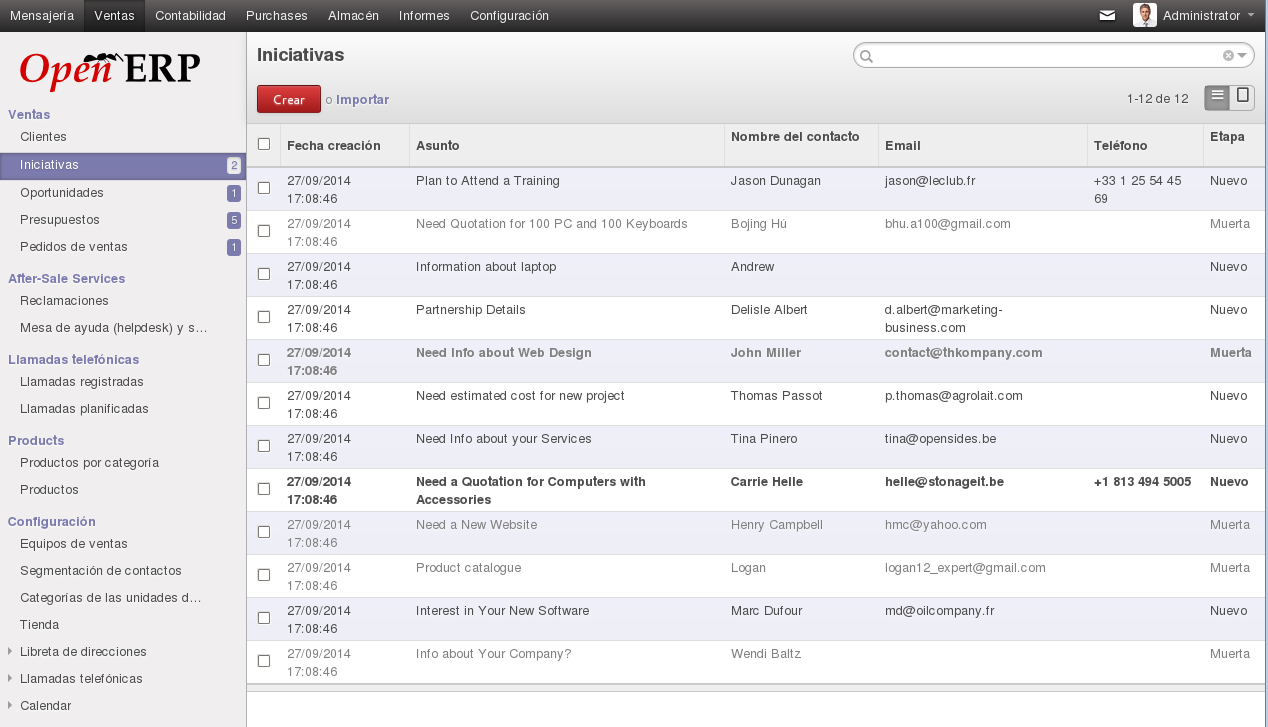
\includegraphics[width=\textwidth]{ventas/img/ven_iniciativas.png}
\caption{Vista de iniciativas}
\label{ven:iniciativas}
\end{figure}

La figura \ref{ven:iniciativas} muestra la vista de las iniciativas al entrar a la misma sección. En la misma se puede apreciar de un
vistazo múltiples iniciativas y sus fechas de creación, nombre del contacto, email y teléfono del mismo. Además, se aprecia el \emph{Asunto} de la 
iniciativa, que corresponde a una breve descripción del asunto a tratar con el cliente. Puede contener una reducida descripción de la posible
venta o algún detalle sobre el contacto.

La \textbf{Etapa} de la iniciativa representa el estado de la misma. Tiene tres posibles estados, aunque uno de ellos no se muestra tal cual (se explica en la descripción del mismo). Estos estados son

\begin{itemize}
  \item \textbf{Nuevo} -- Las iniciativas recien creadas tienen este estado. Se mantienen en este estado hasta que se contacta con el 
                          cliente. Una vez se habla algo con el cliente se pasará la iniciativa a alguno de sus otros estados.
  \item \textbf{Oportunidad} -- Este estado no se mostrará en el listado. Cuando se habla con el cliente relacionado con la iniciativa
                y se puede ver que esta iniciativa, este contacto, puede llevar a alguna venta, se convertirá la iniciativa a oportunidad (mediante el botón \emph{Convertir a oportunidad} que se ve al acceder a la iniciativa).
                En ese momento, se creará una \emph{Oportunidad} en la sección de oportunidades y desaparecerá la iniciativa. Con 
                esto se ha escalado ese contacto a una oportunidad de venta.
  \item  \textbf{Muerta} -- Si tras contactar con el contacto de la iniciativa se aprecia que no existe posibilidad de realizar una venta
               por las razones que sea, se moverá la iniciativa a este estado mediante el botón \emph{Cancelar caso} en la ficha de la 
               iniciativa.
\end{itemize}



\subsubsection{Ficha de iniciativa}

Al hacer click sobre cualquier iniciativa se abrirá la ficha de la misma con toda su información tal como se ve en la figura 
\ref{ven:iniindividual}.

\begin{figure}[H]
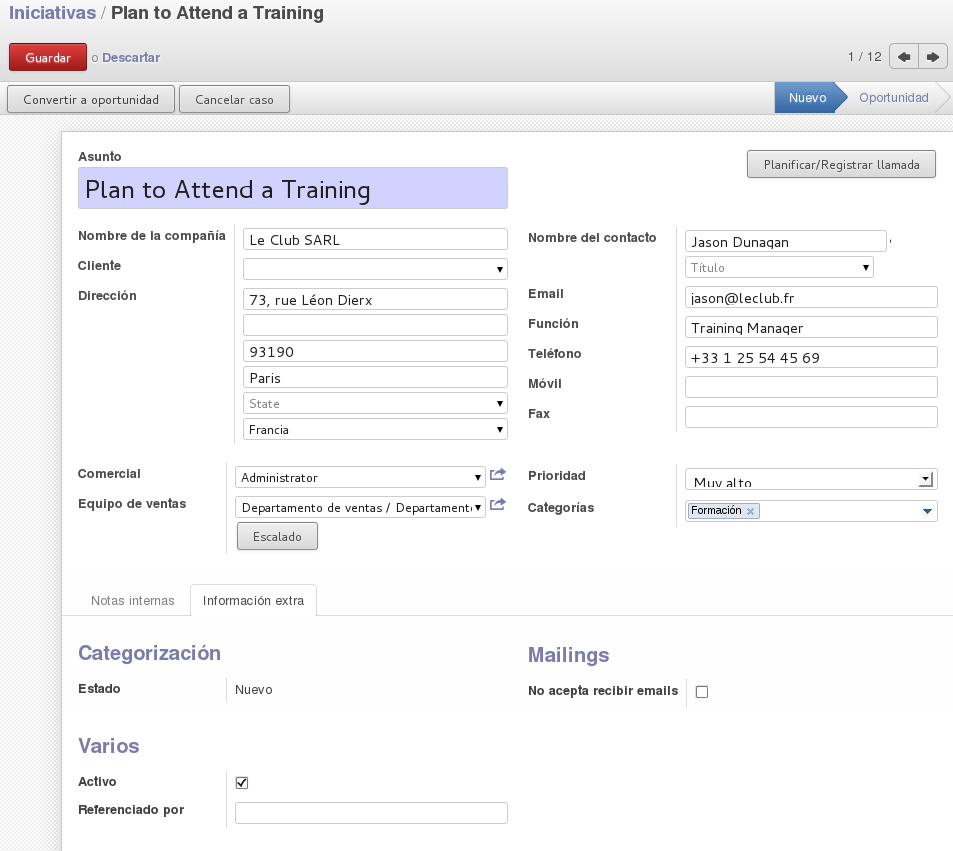
\includegraphics[width=\textwidth]{ventas/img/ven_iniindividual.png}
\caption{Vista de una iniciativa individual}
\label{ven:iniindividual}
\end{figure}

Los datos del contacto se rellenan manualmente. La excepción es si, aunque sea una iniciativa, no es un primer contacto, sino que es un "re-contacto" con un cliente existente, porque el mismo haya mostrado interes o porque se vaya a contactar con él por alguna oferta. En tal caso, eligiendo el cliente adecuado en el campo del mismo nombre, se rellenarán los demás campos de acorde a los datos previamente introducidos del mismo.

A las iniciativas se le pueden asignar distinta \textbf{Prioridad} y varias \textbf{Categorías}, todo ello con caracter de organización interna. Las categorías para ordenar las distintas y las prioridades para agilizar los contactos prioritarios de los que no.

También se puede asignar un \textbf{Comercial} y un \textbf{Equipo de ventas} a las iniciativas. Las iniciativas asignadas a un comercial serán \textbf{vistas sólo por el mismo comercial} al igual que con el equipo de ventas.

Se observa en la parte superior derecha de la ficha de cliente, el botón \emph{Planificar/Registrar llamada}, que permite, como su propio nombre indica, registrar las llamadas hechas/planeadas a ese cliente en relación con esta iniciativa. De las llamadas se habla más concretamente en la sección \ref{llamadas}

Existen dos pestañas en la ficha de iniciativas. La pestaña de \textbf{Notas internas} permite añadir notas de texto a la iniciativa, En el caso de que las iniciativas se creen desde correos electrónicos, esta pestaña contendrá el cuerpo del mensaje recibido.

La pestaña de \textbf{Información extra} contiene la información sobre el \textbf{Estado} de la iniciativa -- vistos anteriormente en el apartado \ref{iniciativas} --, si el cliente \textbf{No acepta recibir emails} y si la iniciativa esta \emph{Activa} y si esta iniciativa está referenciada por alguien.


\subsubsection{Convertir a Oportunidad}
A la hora de convertir a oportunidad la iniciativa, se puede hacer de varias maneras. Al pulsar sobre el botón de conversión a oportunidad, se presentará un dialogo que permitirá elegir distintas opciones -- dialogo representado en la figura \ref{ven:iniaopo}

Por un lado, al convertir a oportunidad puede crearse una nueva oportunidad o fusionarse con una oportunidad ya existente. En el caso de fusionarse con una oportunidad existente, la información de la iniciativa se añadirá a la oportunidad que se indique -- aquella con la que se fusione--.

En el caso de crear una nueva oportunidad, pueden realizarse algunas opciones con los datos del contacto:

\begin{itemize}
  \item \textbf{Crear un nuevo cliente} -- Crea un nuevo cliente con los datos dados. Se muestra la 
        ficha del nuevo cliente para ser completada/confirmada antes de guardar los datos
  \item \textbf{Enlace a un cliente existente} -- Enlaza los datos a un cliente que ya exista para 
        completar los datos que no se tuvieran anteriormente en la ficha del cliente.
  \item \textbf{No enlazar a un cliente} -- Simplemente creará la oportunidad pero no la asociará a 
        ningún cliente.
\end{itemize}

\begin{figure}[H]
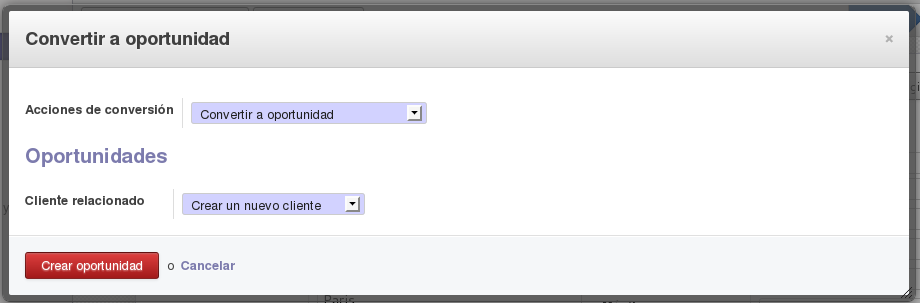
\includegraphics[width=\textwidth]{ventas/img/ven_iniaopo.png}
\caption{Dialogo de conversión de Iniciativa a Oportunidad}
\label{ven:iniaopo}
\end{figure}



\vspace{2cm}
\subsection{Oportunidades}
Mientras que una iniciativa representa un primer contacto con un posible cliente aún por calificar, una oportunidad de venta representa un contrato potencial. Cada oportunidad tiene que ser vigilada por un comercial (o un equipo de ventas) usando su tiempo para calificar la oportunidad, haciendo esto bien a través de una quotation o cancelan la oportunidad.

Las iniciativas son manejadas generalmente por gente diferente, con cierta automatización respondiendo a ciertas entradas o correos. Las oportunidades, por el contrario, son seguidas únicamente por un comercial, debido a que una oportunidad está relacionada con un proceso de negociación con el cliente.

Con las oportunidades, puede administar y realizar el seguimiento del proceso de ventas creando documentos de ventas específicos para cada cliente o cliente potencial. Información como las ganancias esperadas, el estado de la oportunidad, fecha del cierre esperado, historial de comunicación, cuál es la próxima acción y la fecha de la misma y muchas más pueden guardarse en la oportunidad.


\begin{figure}[H]
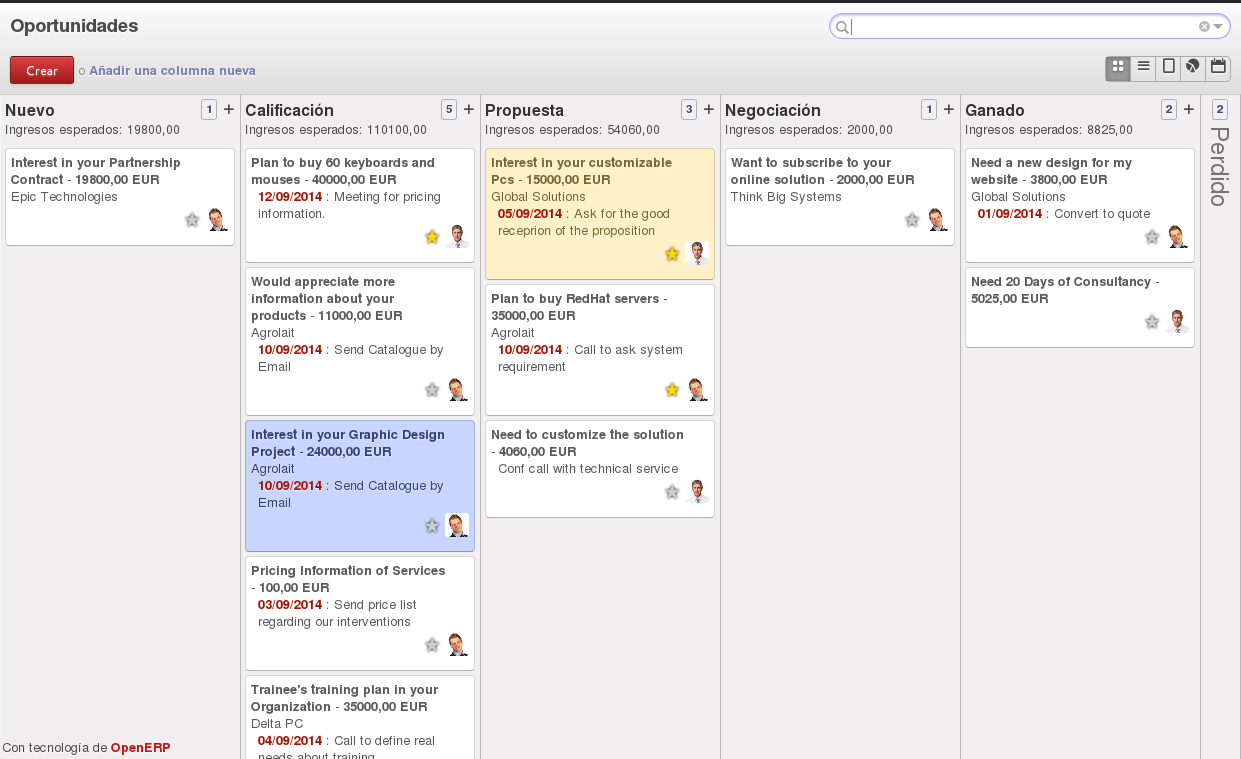
\includegraphics[width=\textwidth]{ventas/img/ven_oportunidades.png}
\caption{Vista Kanban de Oportunidades}
\label{ven:oportunidades}
\end{figure}


\subsubsection{Etapas de las oportunidades}
Al entrar en las oportunidades, se podrá ver una distribución como la mostrada en la figura \ref{ven:oportunidades}. En esta vista tipo 
Kanban, cada columna representa un estado para la oportunidad. Estos estados mostrados por defecto son los \emph{sugeridos} por OpenERP. No obstante, son modificables tanto en número como en nombre, de manera que se adapten más eficientemente al proceso seguido por la empresa.

Estos estados sugeridos por OpenERP pueden entenderse de la siguiente manera:

\begin{description}
   \item[Nueva] -- Estado inicial de las oportunidades. Aquí se sugiere la segmentación de estas oportunidades geográficamente. En este
                punto se hace esa clasificación y se asigna a un comercial. De ahí se pasaría a su siguiente estado.
   \item[Calificación] -- En este punto se trata de que el encargado de la oportunidad atraiga la atenció ndel cliente, determinando 
                las necesidades del mismo. Se trata de encontrar esa necesidad del cliente de comprar un producto o servicio. 
                Cuando esta necesidad está confirmada se da un paso más y se pasa al siguiente estado.
   \item[Propuesta] -- En este momento, el encargado de la oportunidad se encuentra discutiendo con el cliente cuáles son sus necesidades,
                recomendando soluciones específicas para mostrar al cliente. Se espera de esta fase que aparezca una propuesta de compra
                o la necesidad de ver una demo\ldots etc. Se trata de acabar viendo que el cliente tiene interes en la compra.
   \item[Negociación] -- Cuando el cliente muestra interés en la compra se comienza esta fase. Se busca afinar cuál será la compra, las
                condiciones de la misma y el contrato. En esta fase se incluye el envío del contrato para su firma -- o su firma      
                directamente.
   \item[Ganado/Perdido] -- Según la negociación haya llegado a buen o mal puerto, la oportunidad pasará a su estado de ganada
                en el caso de que finalmente el cliente firme por la compra del producto/servicio. Será perdida si finalmente el cliente
                rechaza cualquier tipo de compra o adquisición.
\end{description}

\vspace{2cm}
\subsubsection{Ficha de oportunidad}

\begin{figure}[H]
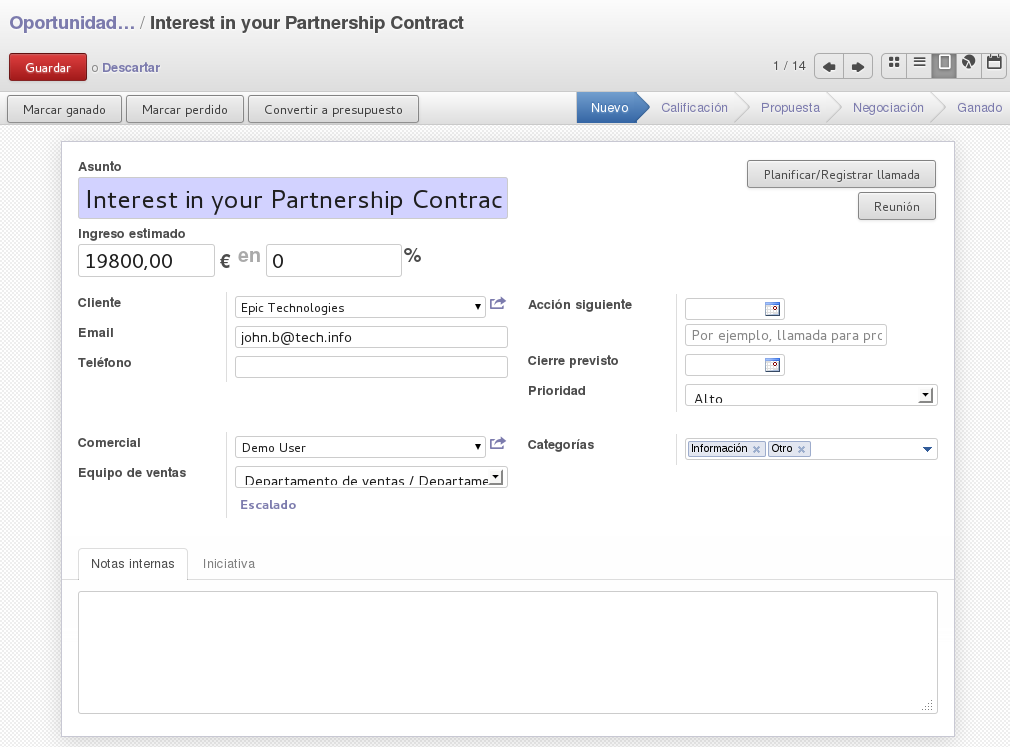
\includegraphics[width=\textwidth]{ventas/img/ven_opoindividual.png}
\caption{Vista de una oportunidad individual}
\label{ven:opoindividual}
\end{figure}

La ficha individual de una \emph{Oportunidad} se puede observar en la figura \ref{ven:opoindividual}. En la parte superior izquierda se 
aprecian unos botones que permiten pasar la oportunidad al estado de \emph{Ganado} o \emph{Perdida} independientemente del estado en el que se encuentre. También se ve un tercer botón que permite pasar la oportunidad directamente a un \textbf{presupuesto}, que marcará, además, la oportunidad como ganada. La información sobre los presupuestos se amplía en el capítulo \ref{presupuestos}.

Al mismo nivel, a la derecha, se pueden observar todos \textbf{los posibles estados} de la Oportunidad. El estado actual se encuentra
marcado en azul. Pulsando sobre los distintos estados podemos variar el estado actual de la oportunidad seleccionada, es la manera 
más sencilla y rápida de cambiar de estado.

Un poco más abajo se pueden observar los botones de \textbf{Planificar/Registrar llamada} y \textbf{Reunión}. El primero sirve para la creación/revisión de las llamadas relacionadas con esta oportunidad, mientras que el de reunión permite crear un nuevo evento en el calendario. Mostrará en primer lugar el calendario y al seleccionar el día rellenará los datos relacionados con el cliente de la reunión
siendo el creador de la reunión el responsable de rellenar el resto de información y de completar quienes serán los asistentes.

El \textbf{Asunto} es una breve descripción de la oportunidad, que será el texto por el que se le identificará cuando se observe la lista de oportunidades. El \textbf{Ingreso estimado} es una aproximación a la cantidad de dinero que se podría obtener con esta oportunidad, y el \textbf{porcentaje} que se situa a su lado es la probabilidad de que la oportunidad acabe en buen puerto. Este porcentaje es hasta cierto punto subjetivo y lo puede rellenar el mismo usuario. Estos datos pueden ser importantes para un análisis de oportunidades y para poder
analizar a posteriori posibles fallos y localizar posibles fallos en el proceso de venta.

Del resto de datos de la ficha cabe recalcar la importancia de los campos \textbf{Acción siguiente}, que permite indicar la fecha en la que
se realizará alguna acción en relación a esta oportunidad y una descripción de este paso (como por ejemplo, la fecha de la próxima llamada y usando como descripción "Llamar con el descuento preparado"). También el campo \textbf{cierre previsto} es importante para calculos
empresariales y hacer un seguimiento más detallado de la venta. Por supuesto que este campo es modificable una vez llegada la fecha,
no se puede estimar el cierre con un 100\% de seguridad, pero con esta información se consigue agilizar el análisis de los movimientos comerciales por parte del encargado de la supervisión de los mismos.

El resto de campos son como los vistos hasta ahora, \textbf{Comercial} y \textbf{Equipo de ventas} refieren al encargado (y su equipo) de
la oportunidad. La \textbf{prioridad} permite ordenar por importancia las oportunidades, y \textbf{Categorías} permite tener organizadas
todas las oportunidades en distintas áreas para supervisarlas independientemente.

La pestaña de \textbf{Notas internas} es, al igual que las vistas anteriormente, un área para guardar información en formato de texto 
plano relacionada con la Oportunidad y la pestaña \textbf{Iniciativa} guarda los datos de contacto y otros introducidos en la Iniciativa
que dió lugar a la oportunidad visualizada. Hay más información sobre los campos de esta pestaña en el capítulo \ref{iniciativas}.


\subsection{Presupuestos}
\label{presupuestos}
Parece innecesario describir un presupuesto a estas alturas. Podemos entenderlo en este punto como una oportunidad que ha sido ganada
y se ha transformado en una venta concreta por confirmar.

Los presupuestos contienen los productos a vender, los datos del cliente y las condiciones de las ventas. En su visión de listado se observan los datos básicos (figura \ref{ven:prelista})
\begin{figure}[H]
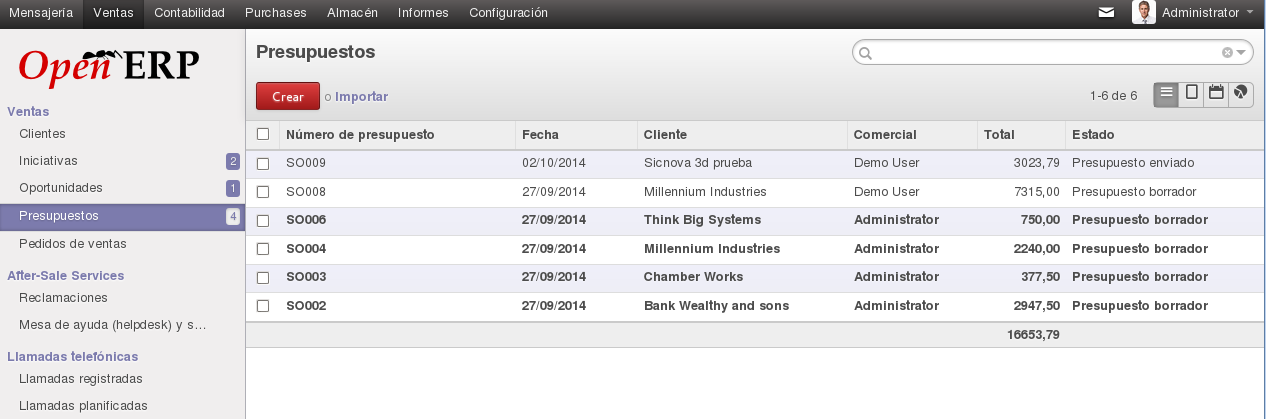
\includegraphics[width=\textwidth]{ventas/img/ven_prelista.png}
\caption{Listado de presupuestos}
\label{ven:prelista}
\end{figure}

La vista del listado es más informativa a nivel general, se puede apreciar en la misma el \textbf{nº del presupuesto}, \textbf{su fecha}, 
\textbf{cliente}, \textbf{comercial} al cargo del presupuesto y el \textbf{total}, que hace referencia al precio total de la venta. Además se aprecia el campo \textbf{estado} que indica en que punto está el presupuesto, sus posibles estados son:

\begin{description}
  \item[Presupuesto borrador] -- Es un presupuesto no confirmado, pendiente de darle el visto bueno y ser enviado al cliente.
  \item[Presupuesto enviado] -- Estado que se alcanza tras el envío del presupuesto al cliente.
  \item[Excepción] -- Este estado se asigna cuando ocurre alguna excepción con el almacén (relacionado con los productos indicados en el
                      presupuesto) o en la factura (la que esté en relación a este presupuesto/orden de venta)
\end{description}
\vspace{1cm}


\subsubsection{Ficha de presupuesto individual}
\begin{figure}[H]
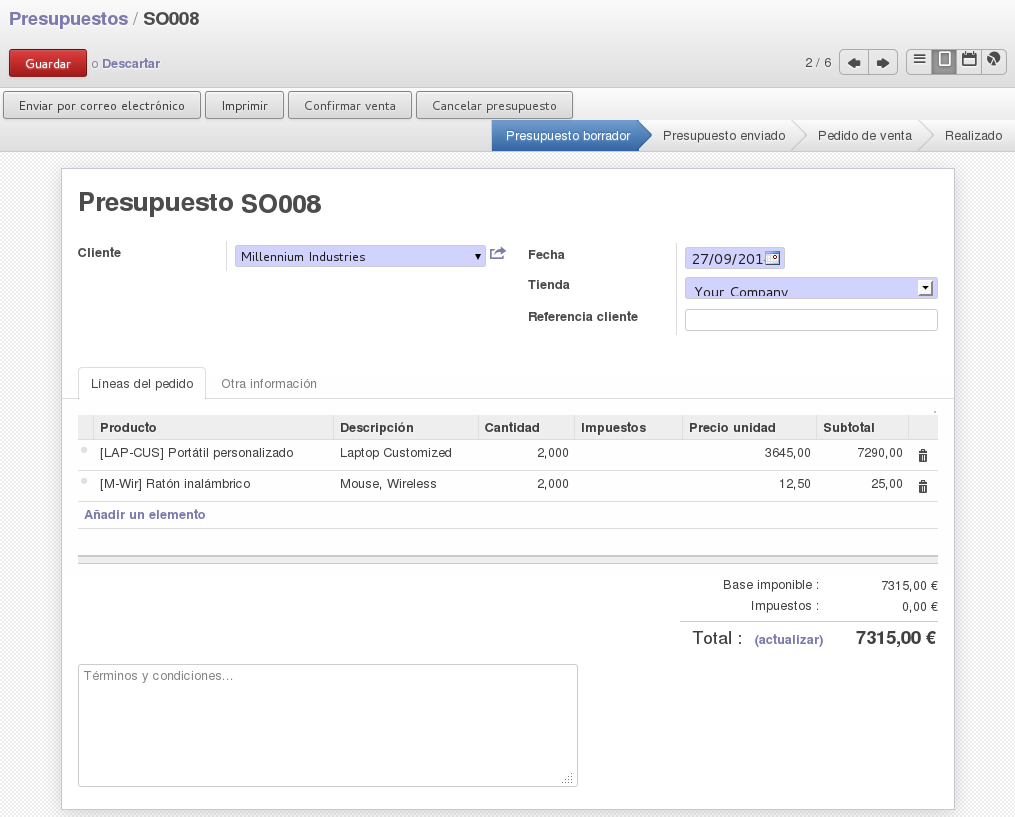
\includegraphics[width=\textwidth]{ventas/img/ven_preindividual.png}
\caption{Ficha individual de presupuesto}
\label{ven:preindividual}
\end{figure}

La figura anterior(\ref{ven:preindividual}) muestra la ficha individual de un presupuesto. Desde la ficha se indica el cliente -- lo que rellenará automáticamente la dirección que se puede apreciar -- la \textbf{fecha de la venta}, la \textbf{tienda} -- habitualmente sólo 
será una y no será necesario cambiarla -- y se puede añadir una \textbf{referencia cliente} a mano.

Las \textbf{líneas de pedido} representan los productos que se venden y se facturan en el presupuesto -- y en la factura final --. Pueden añadirse tantas como sean necesarias. Al seleccionar un nuevo producto, el resto de los elementos de la línea (Descripción, Impuestos, Precio Unidad\ldots) se rellenarán automáticamente con los datos del producto (que se pueden ver en la sección \ref{productos}), pudiendo añadir, eliminar o modificar estas propiedades también aquí si fuera necesario -- se pueden añadir impuestos, modificar el precio \ldots.

Hay que recordar que \textbf{cuando se modifiquen líneas de productos} de un presupuesto, ya seá modificando el número de productos o
variando el impuesto, utilizar la acción \textbf{actualizar} que se puede ver en la línea del total del presupuesto, asegurandose de que se refresca la cantidad y se adapta a los nuevos datos.

Los botones que se observan en la parte superior izquierda de la ficha permiten \textbf{Enviar por correo el presupuesto} directamente al
cliente (o las direcciones que sean necesarias), \textbf{Imprimir} el presupuesto y \textbf{Confirmar la venta} o \textbf{Cancelar el presupuesto}. La confirmación de la venta hará que el presupuesto desaparezca de esta sección y que aparezca en el apartado de \emph{Pedidos de ventas}, el cual se explica en la sección \ref{pedidosventas}

\begin{figure}[H]
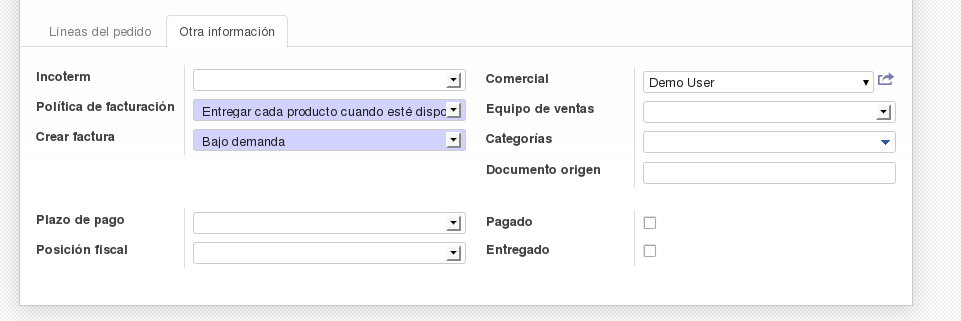
\includegraphics[width=\textwidth]{ventas/img/ven_preindotra.png}
\caption{Pestaña \emph{Otra información} de presupuesto}
\label{ven:preindotra}
\end{figure}

La otra pestaña que se encuentra junto a la de \emph{Líneas de pedido} es \textbf{Otra información}. En ésta (visible en la figura 
\ref{ven:preindotra}). La información obligatoria en este caso es:

\begin{itemize}
  \item \textbf{Política de facturación} -- Permite elegir la política de entrega y facturación de los productos.
  \begin{itemize}
    \item[$\star$] \textbf{Entregar cada producto cuando esté disponible} -- Utilizado para ir sirviendo los productos a medida que se encuentren 
          disponibles en el stock.
    \item[$\star$] \textbf{Entregar todos los productos a la vez} -- Espera a que todos los productos se encuentren disponibles en stock para realizar la
          facturación y envío.
  \end{itemize}

  \item \textbf{Crear factura} -- Indica como se va a realizar la facturación.
    \begin{itemize}
      \item[$\star$] \textbf{Bajo demanda} -- Se crea la factura desde la orden de venta a petición del comercial
      \item[$\star$] \textbf{Sobre la orden de entrega} -- Crea la factura cuando se completa el envío y la entrega de productos al cliente.
      \item[$\star$] \textbf{Antes de la entrega} -- Se crea la factura cuando se confirma el borrador, y no se realiza el envío y entrega de productos hasta
           que la factura esté pagada.
    \end{itemize}
\end{itemize}

Se puede añadir además un \textbf{Plazo de pago} y una \textbf{posición fiscal}, utilizando esta última automáticamente en el área de 
contabilidad, creando los asientos de acuerdo a este elemento también.

El \textbf{Documento de origen} hace referencia al documento original del que deviene este presupuesto, aunque no se utiliza habitualmente puede adaptarse a las necesidad de la empresa.


\subsection{Pedidos de ventas}
\label{pedidosventas}

Los pedidos de ventas son, a nivel de la aplicación, idénticos a los presupuestos salvo que hacen referencia a pedidos de clientes que hay que facturar y enviar, esto es, ventas realizadas. Además, se encuentran en secciones separadas para no ser confundidos con presupuestos, y sus estados son distintos.

\begin{figure}[H]
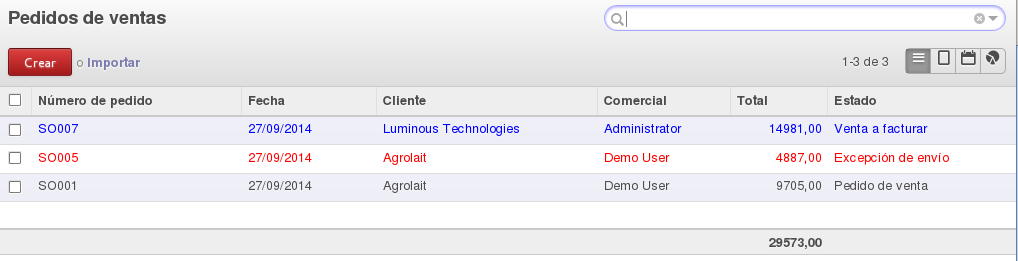
\includegraphics[width=\textwidth]{ventas/img/ven_pedlistado.png}
\caption{Listado de los pedidos de venta}
\label{ven:pedlistado}
\end{figure}

La diferencia básica estriba en la visión individual del pedido de venta tal como se ve en la figura \ref{ven:pedindividual}. En la botonera de la parte superior izquierda se aprecian otros botones con otro texto. En el caso más interesante -- que es cuando la creación de la factura se crea antes del envío -- en el pedido confirmado aparecerá el botón \textbf{Ver factura}. Este botón permite al comercial al cargo del pedido de venta ver la factura del mismo y el estado en el que se encuentra. Aunque el comercial no tenga acceso a la zona de contabilidad, si puede hacer un seguimiento de los documentos relacionados con sus ventas, sólo en modo lectura, es decir, no puede validad ni manipular la factura de ninguna manera, tan solo verla y los datos relacionados con ella.

\begin{figure}[H]
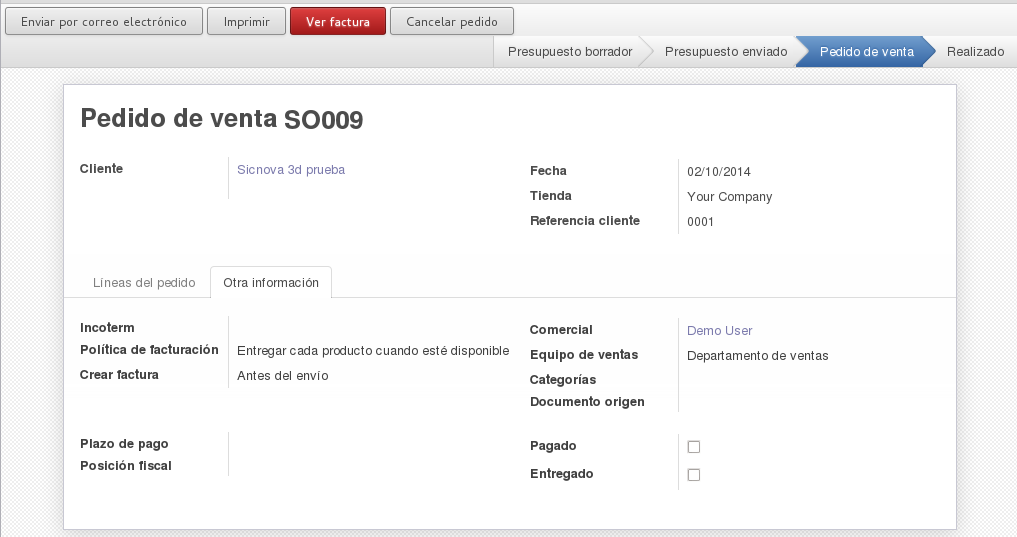
\includegraphics[width=\textwidth]{ventas/img/ven_pedindividual.png}
\caption{Pedido de venta individual}
\label{ven:pedindividual}
\end{figure}

Cuando la factura se registre como pagada en la sección de contabilidad, se creará una orden de envío en el almacén, y aparecerá un nuevo
botón en el pedido de venta, denominado \textbf{Ver orden de entrega}. Este botón, al igual que el de \emph{Ver factura}, permite echar un
vistazo a la orden de envío del almacén, de manera que el comercial puede hacer un seguimiento del envío de su venta. De igual modo que la
factura, sólo puede visualizar la información, no manipularla directamente, ya que de eso se encarga la persona responsable del almacén.




\section{Servicio Post-venta}

Los servicios post-venta se dividen en reclamaciones -- incidencias y problemas que ha habido en una venta/producto -- y peticiones de ayuda (Helpdesk) -- dudas y cuestiones varias por parte de un cliente.

La diferencia básica se encuentra en que las reclamaciones se crean para aceptarlas y solucionarlas o para rechazarlas. Por ejemplo, la
venta de una impresora a la que le faltan las llaves de la puerta sería una reclamación. Esta se acepta, se envían unas llaves y se cierra
la reclamación como resuelta.

Si un cliente tiene una duda sobre un uso concreto poco documentado, éste puede llamar para preguntar y se crearía una entrada en la
sección \emph{Helpdesk}. A partir de aquí el estado de esta pregunta se puede abrir y desarrollar a lo largo del tiempo hasta conseguir
explicarle al cliente esa funcionalidad, crearle un manual\ldots etc. En ese punto se marcaría como resulta.

La diferencia básica está en que las incidencias ocurren y deben ser resueltas en un proceso documentado. Las peticiones de ayuda para helpdesk pueden conllevar una conversación con el cliente y suelen ser preguntas y acciones concretas que no requieren de un desarrollo -- o al menos de un desarrollo extenso -- de su solución. Si se requieriera, estaríamos hablando de una reclamación, una incidencia o fallo
que requiere trabajarla para evitar que se repita.




\subsection{Reclamaciones}

\begin{figure}[H]
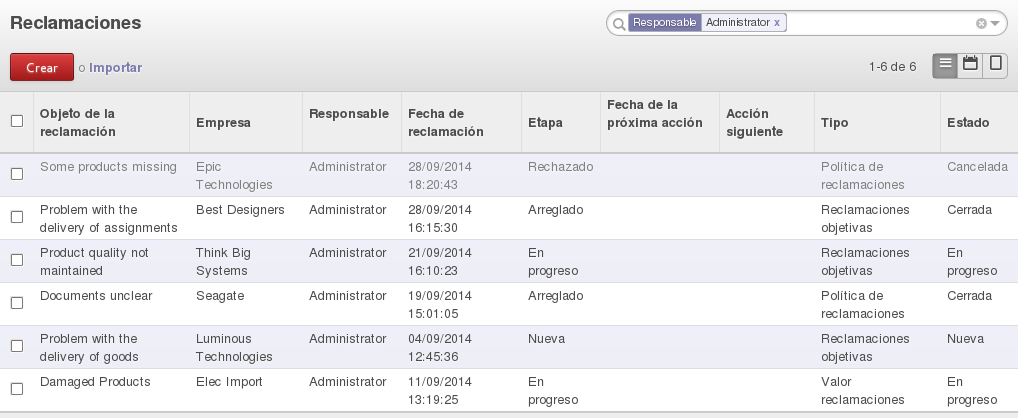
\includegraphics[width=\textwidth]{ventas/img/ven_reclista.png}
\caption{Listado de incidencias}
\label{ven:reclista}
\end{figure}

La figura \ref{ven:reclista} muestra el listado de incidencias, la visión general que se da al entrar en la sección de las mismas. De un
vistazo se pueden ver la información principal. \textbf{Objeto de la reclamación} contendrá un pequeño resumen de la incidencia. En 
\textbf{Empresa} se refleja el cliente que ha generado la incidencia, también se indica el \textbf{Responsable} y \textbf{Fecha de creación}.
La \textbf{Etapa} en la que se encuentra la incidencia. Estas etapas pueden ser:

\begin{description}
  \item[Nueva] -- Cuando se crea la reclamación, este será la etapa que se le asigna por defecto.
  \item[En progreso] -- Si se inician unos trámites que requieran de varios pasos o alargar en el tiempo la incidencia, se le deberá asignar
                     esta etapa. Para poder usar esta etapa habrá que hacer click sobre su nombre en el listado de etapas que figura en la 
                     ficha individual de reclamación, en la parte superior derecha de la misma.
  \item[Arreglado] -- Esta etapa se alcanza cuando se resuelve la reclamación.
  \item[Rechazado] -- Si la reclamación finalmente no resulta como tal, se rechaza y quedará constancia de que esa reclamación realizada
                      por el cliente no es responsabilidad de la empresa.
\end{description} 

La \textbf{Fecha de la próxima acción} y \textbf{Acción siguiente} dan, en este modo de presentar las reclamaciones, una vista rápida del siguiente paso a dar -- el qué y el cuándo -- para resolver la reclamación. El campo \textbf{Estado} representa lo mismo que \textbf{Etapa} en este caso.

\subsubsection{Ficha de reclamación}

\begin{figure}[H]
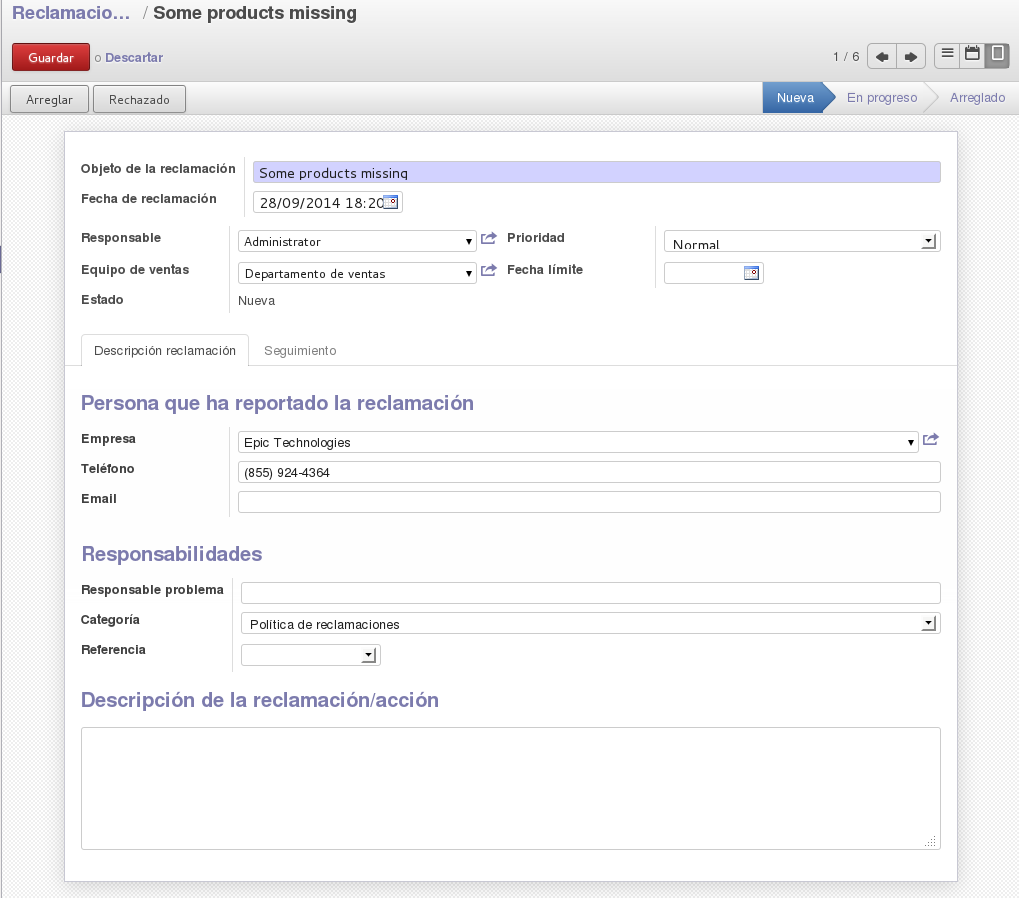
\includegraphics[width=\textwidth]{ventas/img/ven_recindividual.png}
\caption{Ficha de reclamación}
\label{ven:recindividual}
\end{figure}

En la ficha de la reclamación se rellenarán los datos sobre la misma (como se ve en la figura \ref{ven:recindividual}) siendo importante siempre
el utilizar una fecha límite para evitar retrasos en la resolución de problemas. Esta fecha límite debería ser una norma según la empresa que lleve las reclamaciones para evitar problemas que queden sin resolver.

La otra pestaña disponible (\textbf{Seguimiento}) se utiliza para temporizar y hacer el seguimiento detallado del problema expuesto en la
reclamación (figura \ref{ven:recseguimiento})

\begin{figure}[H]
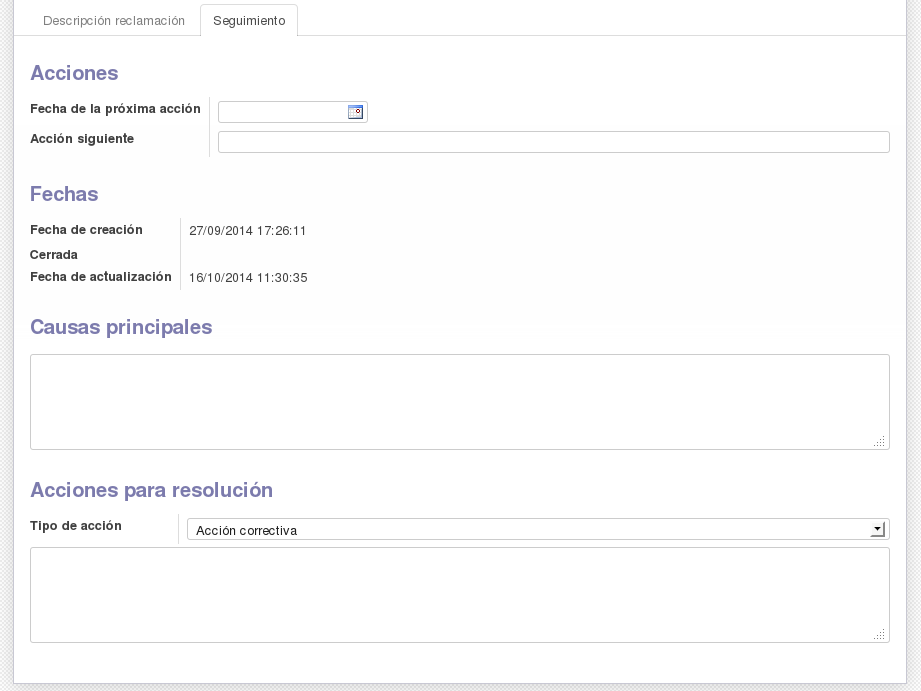
\includegraphics[width=\textwidth]{ventas/img/ven_recseguimiento.png}
\caption{Pestaña de seguimiento en la ficha de reclamación}
\label{ven:recseguimiento}
\end{figure}

Es importante rellenar siempre la \textbf{Acción siguiente} y su \textbf{Fecha de próxima acción} para una gestión eficiente de las 
reclamaciones. El rellenar también las \textbf{Causas principales} y \textbf{Acciones para resolución} ahorrará tiempo en el futuro, tanto
al encargado de resolver la reclamación como a cualquier otro que requiera intervenir en la misma, además de ofrecer información sobre
los problemas que se van encontrando al supervisor del área.

\subsection{Helpdesk}
A continuación, en la figura \ref{ven:hellistado} se muestra la vista en forma de lista de las peticiones de ayuda.

\begin{figure}[H]
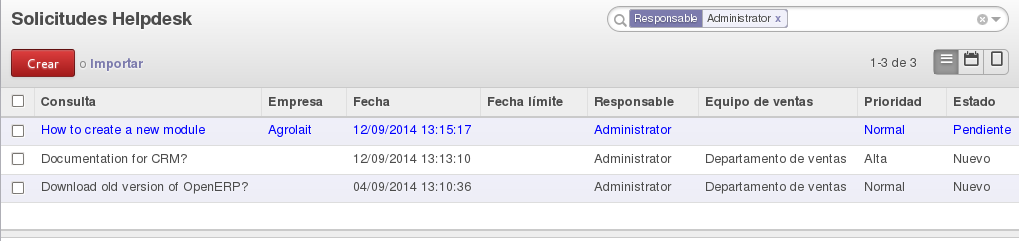
\includegraphics[width=\textwidth]{ventas/img/ven_hellistado.png}
\caption{Listado de peticiones de ayuda (helpdesk)}
\label{ven:hellistado}
\end{figure}

De igual modo que en las reclamaciones, aquí se ofrece una visión generalizada de las peticiones existentes y una descripción breve
de las mismas. Se observa una distribución distinta de los campos a pesar de que la información que muestran es la misma. La \textbf{Fecha límite} es igual de importante que cuando se mencionó en las reclamaciones.

\subsubsection{Ficha de Helpdesk}

\begin{figure}[H]
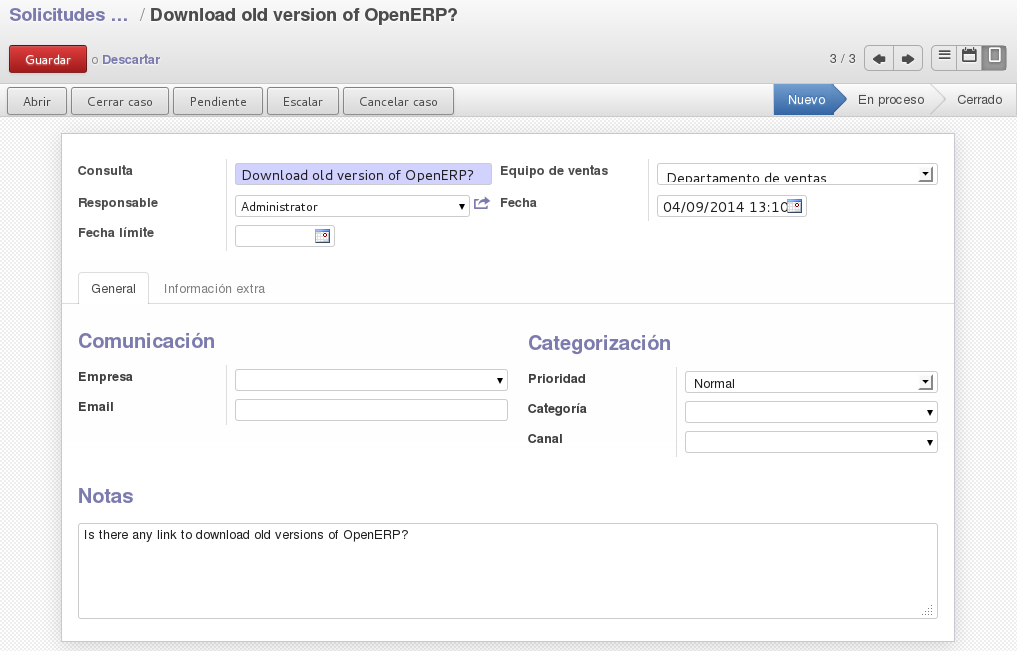
\includegraphics[width=\textwidth]{ventas/img/ven_helindividual.png}
\caption{Ficha individual de Helpdesk}
\label{ven:helindividual}
\end{figure}

La ficha de Helpdesk individual mostrada en la figura superior (\ref{ven:helindividual}) muestra los detalles de la petición de ayuda.
La sección \textbf{Comunicación} se utiliza para introducir los datos de la empresa/cliente que genera la petición de ayuda. En \textbf{Categorización} se clasifica la petición en categorías y prioridades. También se le puede asignar un \textbf{Canal}, que hace referencia
al canal por el cuál ha llegado la petición -- algunos ejemplos son: por email, teléfono, a través de web\ldots --. Y por supuesto en el apartado de \textbf{Notas} se detalla la petición de ayuda con más detalle.

En la pestaña de \textbf{Información extra} (figura \ref{ven:helextra}) pueden añadirse \textbf{Referencias} como la empresa que generó la consulta, una factura relacionada, eventos, números de serie\ldots Al igual que añadir si va a llevar algún coste resolver esta duda para poder facturarlo a posteriori.

\begin{figure}[H]
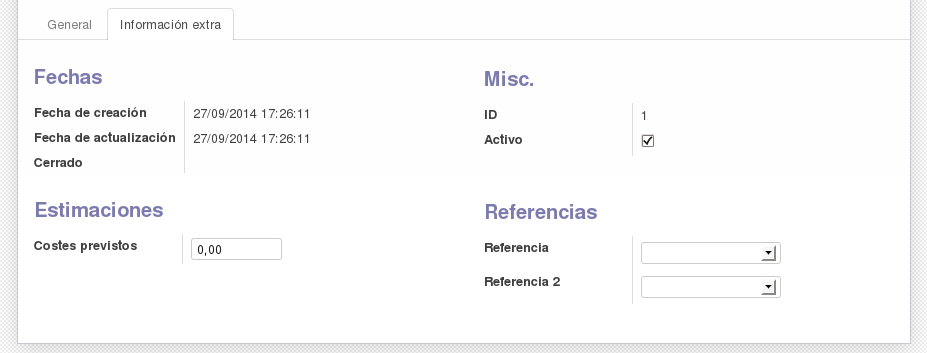
\includegraphics[width=\textwidth]{ventas/img/ven_helextra.png}
\caption{Pestaña \emph{Información extra} de Helpdesk}
\label{ven:helextra}
\end{figure}




\section{LLamadas telefónicas}
\label{llamadas}

Con las llamadas se puede tener un control informativo sobre los contactos hechos a través de teléfono con clientes y/o clientes potenciales. También para organizar comercialmente las llamadas, pudiendo planificar llamadas, extraer conclusiones y generar reuniones, todo directamente desde esta sección.

Hay dos tipos de llamadas en el software. Unas son las \textbf{llamadas registradas} que son aquellas que se registran como ya hechas, a cliente contactado, y las \textbf{llamadas planificadas}

\subsection{Llamadas registradas}
Las llamadas realizadas las conforman el registro de llamadas ya hechas a clientes. Es una sección sencilla, la única visión es en forma
de lista como se ve en la figura \ref{ven:llarealizadas}.

\begin{figure}[H]
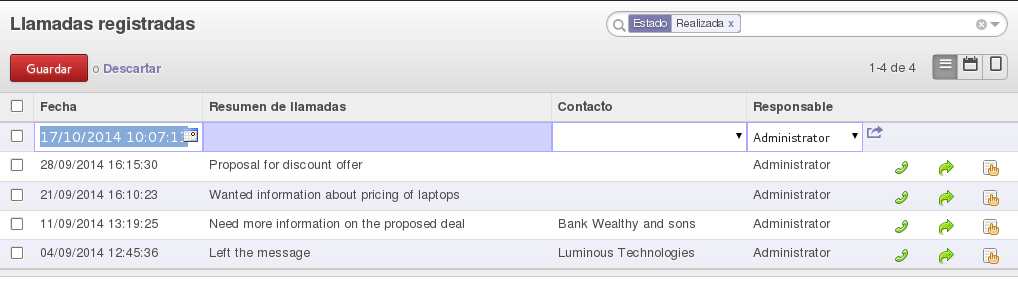
\includegraphics[width=\textwidth]{ventas/img/ven_llarealizadas.png}
\caption{Listado de llamadas realizadas}
\label{ven:llarealizadas}
\end{figure}

Los campos resultan bastante intuitivos, la \textbf{fecha}, el \textbf{Resumen de llamadas}, \textbf{Contacto} y \textbf{Responsable} se 
completaran con los datos descritos por el mismo campo. En el caso del \emph{Contacto} se puede realizar la busqueda del cliente a través
del desplegable, al igual que del \textbf{Responsable}.

En la parte derecha de cada llamada registrada hay tres iconos que permiten distintas acciones a partir de la información de la llamadas, son los siguientes:

\begin{itemize}
  \item \textbf{Teléfono} -- Con este botón se puede generar una nueva llamada registrada o planificar una nueva llamada. Al pulsarlo se 
                           abrirá una ventana con los datos rellenados -- y modificables por el que esté creando esta nueva llamada -- en 
                           un diálogo que se puede ver en la figura \ref{ven:llacrear}
  \item \textbf{Flecha verde} -- Crea una nueva reunión a partir de la llamada. Al pulsar, se abrirá la visión del calendario, donde se 
                           podrá pinchar en cualquier día para crear ahí la nueva reunión. Al pulsar sobre el día se abrirá un dialogo 
                           complementario para introducir todos los datos de la reunión.
  \item \textbf{Icono de la mano} -- Convierte la llamada en una oportunidad. Crea la oportunidad y automáticamente introduce los datos
                           del contacto -- los que hubiera en la llamada -- en la oportunidad. El resto de datos puede introducirlos o
                           modificarlos el usuario.
\end{itemize}

\begin{figure}[H]
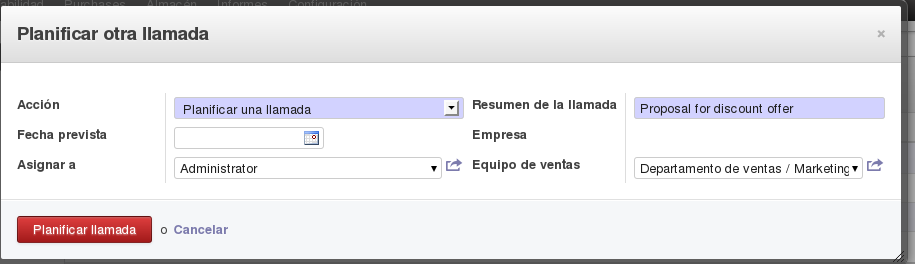
\includegraphics[width=\textwidth]{ventas/img/ven_llacrear.png}
\caption{Diálogo para crear una nueva llamada a partir de una registrada}
\label{ven:llacrear}
\end{figure}




\subsection{Llamadas planificadas}

Estas llamadas son las que están por realizar. La vista principal al entrar en esta sección es en forma de lista (figura \ref{ven:llaplanificadas}). Los campos que coinciden en nombre con los descritos en las llamadas realizadas cumplen las mismas funciones,
\textbf{Fecha}, \textbf{Resumen de llamada}, \textbf{contacto}, \textbf{teléfono} y \textbf{responsable} no necesitan una descripción más allá de su propio nombre.

En el caso del \textbf{Estado} sólo podrá ser \emph{Confirmado}, refiriendos a que la llamada está creada y confirmada, y \emph{Realizada}, una vez hecha. En ese punto, la llamada se moverá automáticamente al listado de llamadas realizadas. Si se \emph{cancela} una llamada puede alcanzar un estado del mismo nombre. La llamada cancelada se verá en gris, no desaparece del todo para, en caso necesario, volver a activarla.

\begin{figure}[H]
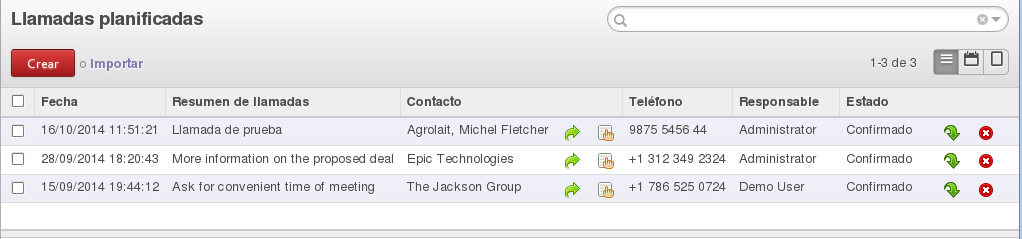
\includegraphics[width=\textwidth]{ventas/img/ven_llaplanificadas.png}
\caption{Diálogo para crear una nueva llamada a partir de una registrada}
\label{ven:llaplanificadas}
\end{figure}

Al igual en las llamadas realizadas, aquí se aprecian algunos iconos que dotan de acciones extra a las llamadas. En el area central se
pueden apreciar dos iconos, identicos en aspecto y funcionalidad a los vistos en las llamadas registradas, en este caso son dos en lugar 
de tres y son:

\begin{itemize}
  \item \textbf{Flecha verde} -- Crea una nueva reunión a partir de la llamada. Al pulsar, se abrirá la visión del calendario, donde se 
                           podrá pinchar en cualquier día para crear ahí la nueva reunión. Al pulsar sobre el día se abrirá un dialogo 
                           complementario para introducir todos los datos de la reunión.
  \item \textbf{Icono de la mano} -- Convierte la llamada en una oportunidad. Crea la oportunidad y automáticamente introduce los datos
                           del contacto -- los que hubiera en la llamada -- en la oportunidad. El resto de datos puede introducirlos o
                           modificarlos el usuario.
\end{itemize}

Además de estos, hay dos iconos más en la parte derecha de cada elemento de la lista de llamadas planificadas:

\begin{itemize}
  \item \textbf{Flecha verde hacia abajo} -- Indica que la llamada ha sido realizada. Convierte la llamada planificada en realizada y 
                           la pasa automáticamente al listado de llamadas realizadas.
  \item \textbf{Circulo rojo con X} -- Cancela la llamada, pasandola a su estado de \emph{Cancelada}.
  \item \textbf{Figuras geométricas con una flecha} -- Este icono sólo aparece cuando la llamada está en el estado de \emph{Cancelada}.
                           su función es pasar la llamada de nuevo a \emph{para hacer}, reactivandola y devolviendola al estado de 
                           confirmada. Cuando aparece este icono -- al estar en el estado de cancelada -- los demás iconos, a excepción 
                           del de crear una oportunidad a través de la llamda, desaparecen.
\end{itemize}


\subsubsection{Ficha de llamada planificada}

\begin{figure}[H]
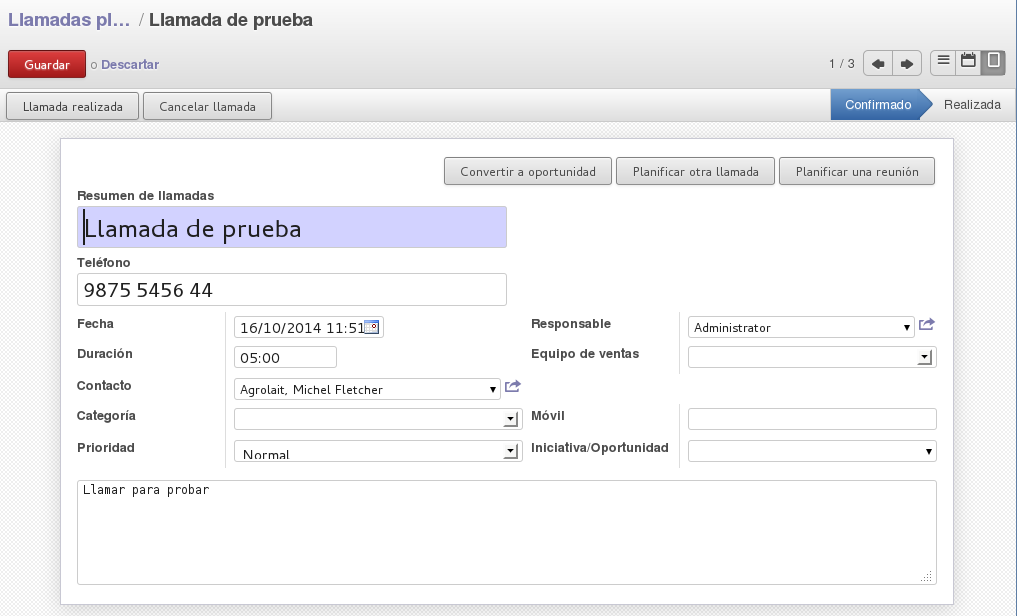
\includegraphics[width=\textwidth]{ventas/img/ven_llaindividual.png}
\caption{Ficha de una llamada planificada}
\label{ven:llaindividual}
\end{figure}

En la imagen superior (figura \ref{ven:llaindividual}) se observa la ficha de una llamada planificada. La zona superior, habilitada con
múltiples botones, realizan las funciones que se han visto en los iconos que aparecen en las llamadas cuando se ve en forma de listado.

Los campos son los mismos que los vistos hasta ahora. Con \textbf{Categoría} y \textbf{Prioridad} se puede realizar la clasificación 
vista en otras secciones para organizar y gestionar correctamente las llamadas. El \textbf{Responsable} y \textbf{Equipo de ventas} clasifican las llamadas de manera que cada usuario de esta sección pueda ver sólo las llamadas de las que es responsable y, a la vez, dar
una estructura de permisos para generar supervisores más o menos generales de las llamadas.

El campo \textbf{Iniciativa/Oportunidad} sirve para relacionar la llamada que se está creando con una iniciativa u oportunidad ya existente. Asociandolas de esta manera se podrá, después, acceder desde la iniciativa u oportunidad a esta y las demás llamadas relacionadas con ella, pudiendo hacer un seguimiento de como se ha tratado esa inciativa/oportunidad por parte del responsable.

%\section{Productos}
